\section{BlaBlaCar}
\label{chap:blablacar}

Tak, jak na své úvodní stránce BlaBlaCar uvádí:

\begin{center}
\textit{BlaBlaCar je přední světová komunita spolujízdy, která spojuje řidiče a cestující na stejné trase, a umožňuje tak levné meziměstské cestování.}
\end{center}

Na základě tohoto jednoduchého principu si lidé mohou přisednout k někomu jako spolucestující. Tímto způsobem se tak dostanou k častokrát levnější a pohodlnější formě přepravy. Pro řidiče je výhodou částečné proplacení jízdy (pohonných hmot) těmito spolucestujícími.\\

Postupně projdu každou, pro mě důležitou stránku, webu BlaBlaCar a u každé takové stránky definuji seznamy pozitivních a negativních vlastností.

\subsection{Hlavní stránka}
Viz obrázek \ref{fig:blablacar:homepage}.
\begin{figure}[h]
    \centering
    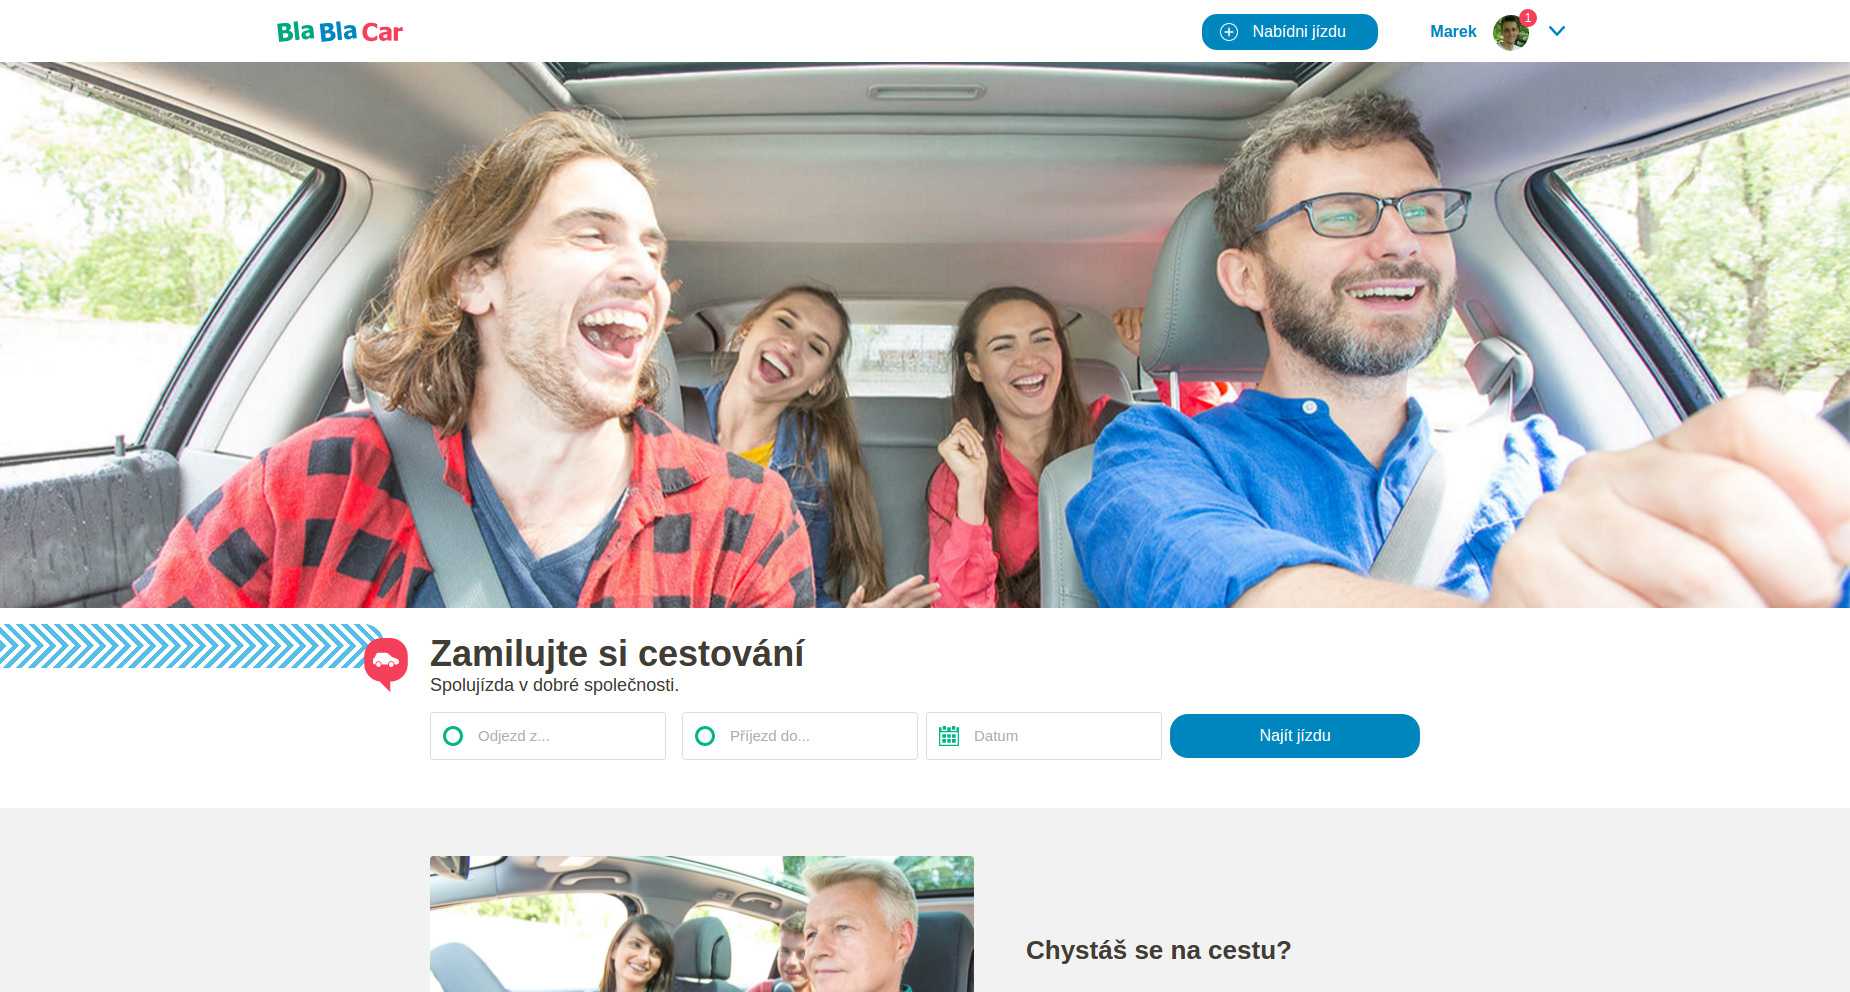
\includegraphics[width=1.0\textwidth]{media/blablacar/homepage.png}
    \caption{Hlavní stránka webu BlaBlaCar.cz}
    \label{fig:blablacar:homepage}
\end{figure}
\subsubsection*{Pozitiva}
\begin{itemize}
    \item[+] \textbf{Přehlednost} -- Na stránce jsou výrazně viditelné dva nejdůležitejší typy úkonů a to \textit{Nabídnutí jízdy} a \textit{Vyhledávání jízdy}. I v mém návrhu budu brát ohled na to, aby každá důležitá akce měla nejvyšší prioritu.
    \item[+] \textbf{Ostatní možnosti} -- V pravém horním rohu je dostupný profil uživatele stejně jako nové upozornění na události týkajících se uživatelského profilu.
    \item[+] \textbf{Jak to funguje} -- Každému uživateli na první pohled nemusí být jasné, o co se přesně jedná. Proto web BlaBlaCar.cz na své úvodní stránce uvádí postup jak se na spolujízdu registrovat.
    \item[+] \textbf{Oblíbené trasy} -- Seznam tří uživateli nejoblíbenějších tras.
\end{itemize}
\subsubsection*{Negativa}
\begin{itemize}
    \item[-] \textbf{Nejoblíbenější řidič} -- Uvítal bych možnost rychlého přístupu k řidiči, se kterým vykonávam většinu jízd.
\end{itemize}


%%%%%%%%%%%%%%%%%%%%%%%%%%%%%%%%%%%%%%%%%%%%%%%%%%%%%%%%%%%%%%%%%%%%%%%%%%%%%%%%%%%%%%%%%%%%%%%%%%%%%%%%%%%%%%%%%%%%%%%%

\newpage
\subsection{Vyhledávání jízdy}
Viz obrázek \ref{fig:blablacar:search}.
\begin{figure}[h]
    \centering
    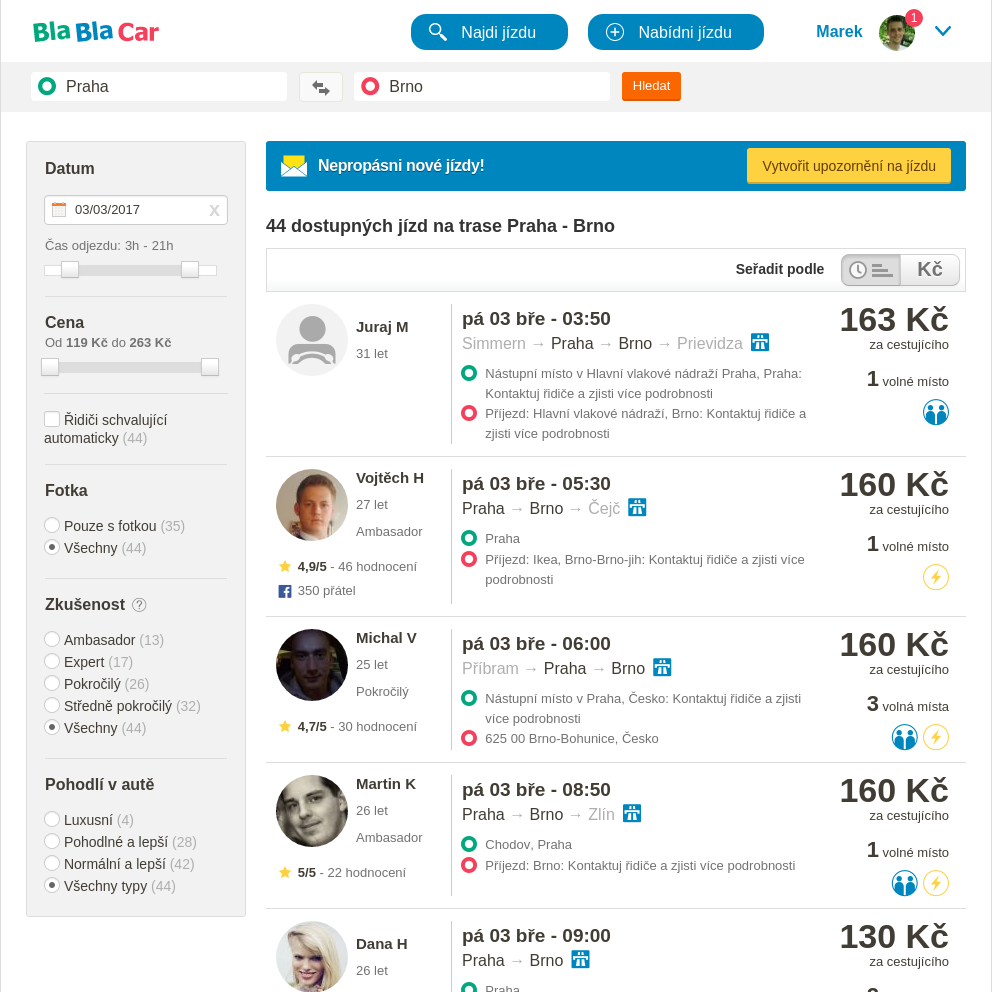
\includegraphics[width=1.0\textwidth]{media/blablacar/search.png}
    \caption{Vyhledávání nabídek na webu BlaBlaCar.cz}
    \label{fig:blablacar:search}
\end{figure}
\subsubsection*{Pozitiva}
\begin{itemize}
    \item[+] \textbf{Informativnost} -- Hned na první pohled uživatel vidí všechny relevantní informace: čas, cena, počet volných míst, délku trasy, hodnocení daného řidiče.
    \item[+] \textbf{Filtry} -- Možnost filtrovaní požadavků na základě zkušeností řidiče a pohodlí auta považuji za nejzajímavější.
    \item[+] \textbf{Možnost řazení} -- Seřazení nabídek podle ceny a času odjezdu je určite velmi potřebná vlastnost.
\end{itemize}
\subsubsection*{Negativa}
\begin{itemize}
    \item[-] \textbf{Nedostupnost profilu řidiče na jeden klik} -- Na první pohled očakávaná funkcionalita (existence předělu mezi cestou a profilem řidiče), při které by se uživatel po kliknutí myší na pravou čast nabídky dostal na bližší informace o jízdě a po kliknutí na levou čast nabídky dostal na profil řidiče. Tohoto problému se při návrhu uživatelského rozhraní budu snažit vyvarovat.
\end{itemize}


%%%%%%%%%%%%%%%%%%%%%%%%%%%%%%%%%%%%%%%%%%%%%%%%%%%%%%%%%%%%%%%%%%%%%%%%%%%%%%%%%%%%%%%%%%%%%%%%%%%%%%%%%%%%%%%%%%%%%%%%

\newpage
\subsection{Detail jízdy}
Viz obrázek \ref{fig:blablacar:detail}.
\begin{figure}[h]
    \centering
    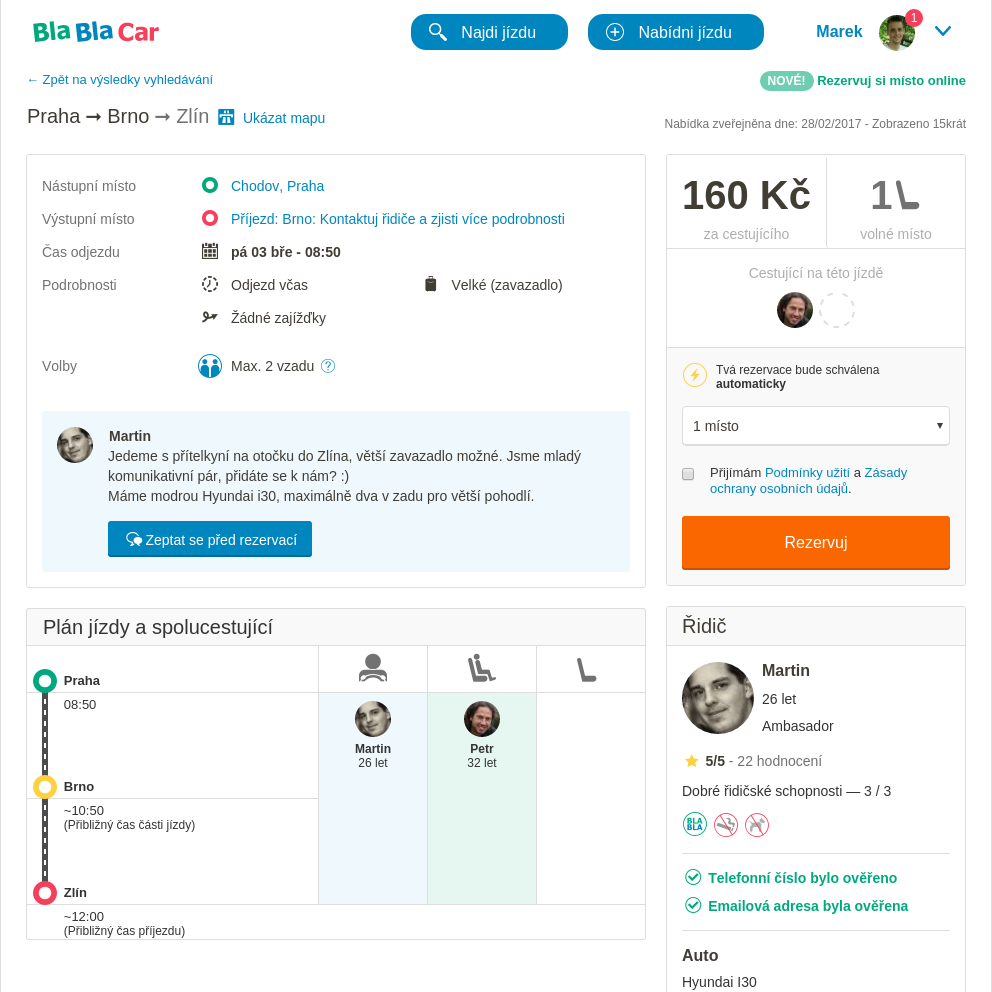
\includegraphics[width=1.0\textwidth]{media/blablacar/detail.png}
    \caption{Detail jízdy na webu BlaBlaCar.cz}
    \label{fig:blablacar:detail}
\end{figure}
\subsubsection*{Pozitiva}
\begin{itemize}
    \item[+] \textbf{Harmonogram} -- Graficky velmi pěkně řešený přehled celé jízdy a spolucestujících včetně časů odjezdů a příjezdů.
    \item[+] \textbf{Spolucestující} -- Možnost vidět kdo s vámi cestuje je vítaná, jelikož s někým se rádi svezete a někomu se naopak raději vyhnete.
    \item[+] \textbf{Podrobnosti} -- Tímto se řidič vyhne nepříjemnostem s velkým počtem zavazadel a uživatel s delšími zajížďkami řidiče.
\end{itemize}
\subsubsection*{Negativa}
\begin{itemize}
    \item[-] \textbf{Žádná negativa na této stránce nevidím.}
\end{itemize}


%%%%%%%%%%%%%%%%%%%%%%%%%%%%%%%%%%%%%%%%%%%%%%%%%%%%%%%%%%%%%%%%%%%%%%%%%%%%%%%%%%%%%%%%%%%%%%%%%%%%%%%%%%%%%%%%%%%%%%%%

\newpage
\subsection{Nabídnutí jízdy}
Viz obrázky \ref{fig:blablacar:offer} a \ref{fig:blablacar:offer2}.
\begin{figure}[h]
    \centering
    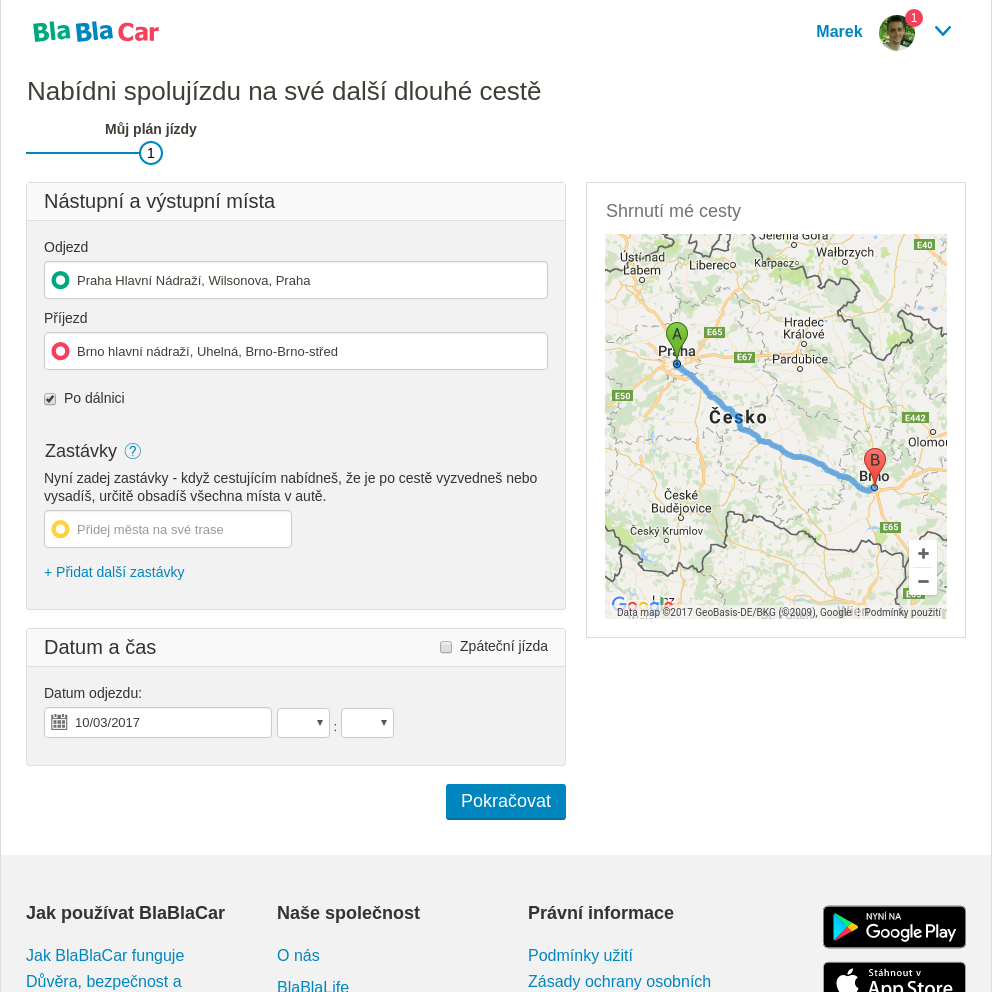
\includegraphics[width=1.0\textwidth]{media/blablacar/offer.png}
    \caption{Zadání nové jízdy na webu BlaBlaCar.cz - Harmonogram}
    \label{fig:blablacar:offer}
\end{figure}
\begin{figure}[h]
    \centering
    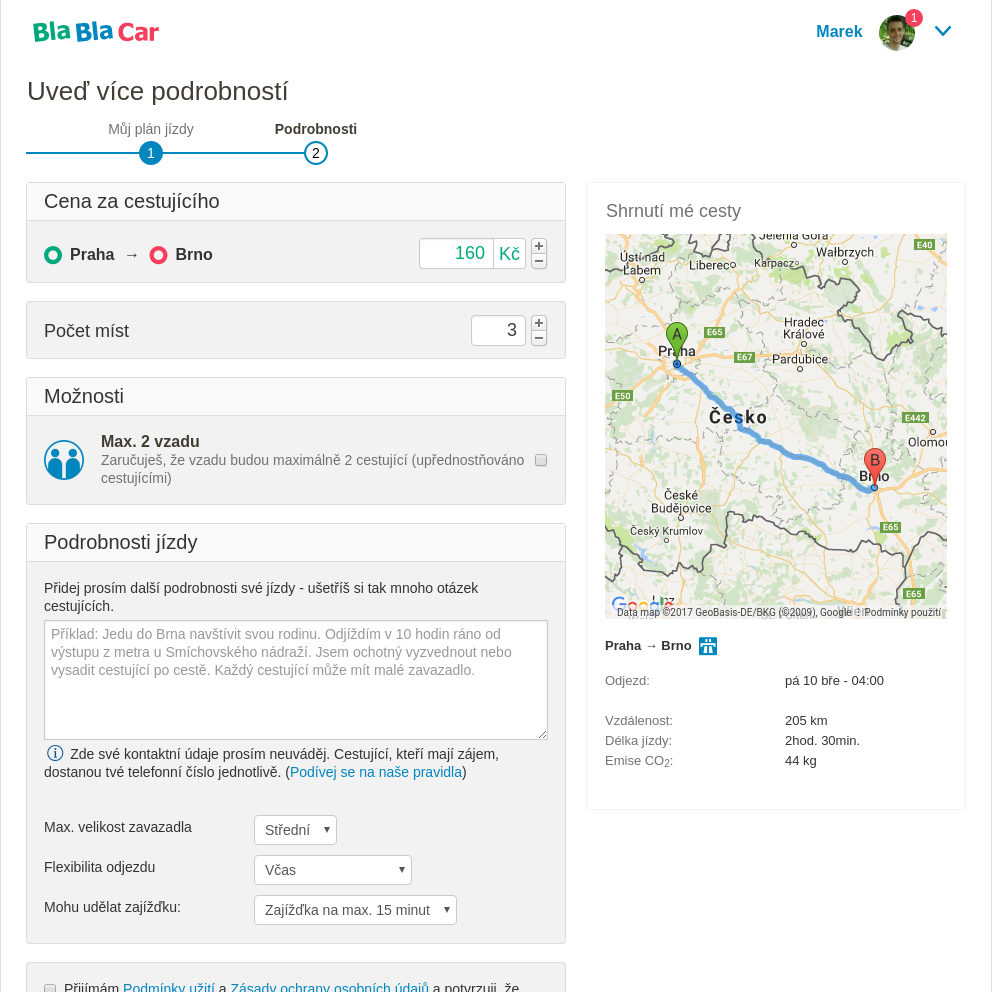
\includegraphics[width=1.0\textwidth]{media/blablacar/offer2.png}
    \caption{Zadání nové jízdy na webu BlaBlaCar.cz - Podrobnosti}
    \label{fig:blablacar:offer2}
\end{figure}
\subsubsection*{Pozitiva}
\begin{itemize}
    \item[+] \textbf{Krok za krokem} -- Uživatel postupně prochází všemi důležitými aspekty nabídky jízdy.
    \item[+] \textbf{Přijatelné UI} -- Všechno je na svém místě a výrazně odlišené od ostatních položek.
    \item[+] \textbf{Doporučená cena} -- Automatické vyplnění ceny na základě ostatních nabídek a vzdálenosti.
    \item[+] \textbf{Mapa} -- Mapa i celkové shrnutí vzdálenosti a trvání jízdy. Speciálně zajímavým prvkem se mi jeví množství emisí vypuštěných do ovzduší.
\end{itemize}
\subsubsection*{Negativa}
\begin{itemize}
    \item[-] \textbf{Nevidím}
\end{itemize}


%%%%%%%%%%%%%%%%%%%%%%%%%%%%%%%%%%%%%%%%%%%%%%%%%%%%%%%%%%%%%%%%%%%%%%%%%%%%%%%%%%%%%%%%%%%%%%%%%%%%%%%%%%%%%%%%%%%%%%%%

\newpage
\subsection{Profil uživatele}
Viz obrázek \ref{fig:blablacar:profile}.
\begin{figure}[h]
    \centering
    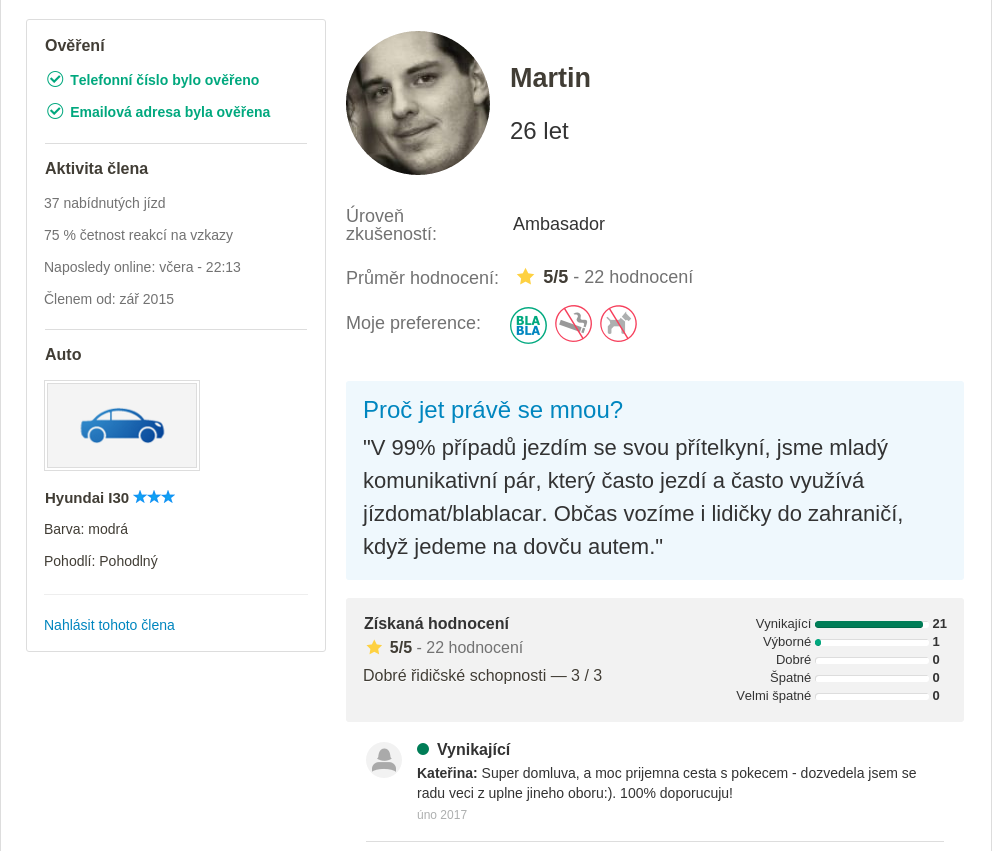
\includegraphics[width=1.0\textwidth]{media/blablacar/profile.png}
    \caption{Profil uživatele na webu BlaBlaCar.cz}
    \label{fig:blablacar:profile}
\end{figure}
\subsubsection*{Pozitiva}
\begin{itemize}
    \item[+] \textbf{Informativnost} -- Recenze, typ auta, počet nabídnutých jízd. Jednoduše se dozvíme vše co potřebujeme bez nutnosti přecházet na další stránku
    \item[+] \textbf{Ověření} -- Různé úrovně ověření každého uživatele. Tuto funkcionalita se mi líbí a zvážím její přidání do mé aplikace.
\end{itemize}
\subsubsection*{Negativa}
\begin{itemize}
    \item[-] \textbf{Nevidím}
\end{itemize}


%%%%%%%%%%%%%%%%%%%%%%%%%%%%%%%%%%%%%%%%%%%%%%%%%%%%%%%%%%%%%%%%%%%%%%%%%%%%%%%%%%%%%%%%%%%%%%%%%%%%%%%%%%%%%%%%%%%%%%%%

\newpage
\subsection{Shrnutí}
Pro účel aplikace jsou nejdůležitější dvě stránky, které BlaBlaCar poskytuje a to: \textbf{Vyhledávání jízdy} a \textbf{Detail jízdy}.

Při návrhu uživatelského rozhraní se zaměřím na poskytnutí možnosti filtrování a také seřazení nabídek. Zakomponuji rozdílnost kliknutí na uživatele, která uživatele dostane na jeho profil, resp. samotné nabídky, která nás přesměruje na bližší informace o dané nabídce.

I napříč tomu, že v moji aplikaci neexistují \textbf{spolucestující}, tak si beru příklad z této vlastnosti BlaBlaCar a při detailech nabídky zvážím výpis historie s daným uživatelem, která slouži velmi podobnému účelu.

Hodnocení uživatelů je řešeno pomocí pěti-hvězdičkového systému.